\documentclass[12pt]{beamer}

\hypersetup{colorlinks=true,linkcolor=red}
\usetheme{default}
\usecolortheme{albatross}

\usepackage[utf8]{inputenc}
\usepackage[russian,english]{babel}
\usepackage[T2A]{fontenc}
\usepackage{hyperref}
\usepackage[final]{listings}
\usepackage{breakurl}
\usepackage{cite}
\usepackage{perpage}

\graphicspath{{img/}}

\def\Url\Breaks{\do\/\do-}
\lstset{
  frame=single,
  breaklines=true,
  basicstyle=\tiny,
  postbreak=\raisebox{0ex}{\ensuremath{\hookrightarrow\space}},
  numbers=left
}

\lstdefinestyle{base}{
  frame=single,
  breaklines=true,
  basicstyle=\tiny,
  postbreak=\raisebox{0ex}{\ensuremath{\hookrightarrow\space}},
  moredelim=[is][\color{red}]{@}{@},
  numbers=left
}

\MakePerPage{footnote}

\title{Operating Systems}
\subtitle{File Systems}
\author{Me}
\date{\today}

\begin{document}
  \begin{frame}
    \titlepage
  \end{frame}

  \begin{frame}
\frametitle{Файловая система}
\begin{itemize}
  \item Блочные устройства позволяют хранить большие объемы информации долгое
  время
  \begin{itemize}
    \item чем больше информации тем больше хочется ее структурировать.
  \end{itemize}
  \item Multics впервые (*) ввел в использование иерархическую файловую систему:
  \begin{itemize}
    \item файлы, каталоги/директории/папки, жесткие и символьные ссылки;
    \item так как Multics пофейлился, популярной иерархиеские ФС сделал скорее
    Unix.
  \end{itemize}
\end{itemize}
\end{frame}

\begin{frame}
\frametitle{Операции над файлами}
\begin{itemize}
  \item открытие файла - возвращает некоторый дескриптор, который используется
  для дальнейших операций с файлами
  \begin{itemize}
    \item снаружи этот дескриптор обычно выглядит просто как целое число;
    \item внутри ОС это обычно некоторая структура, которая кеширует информацию
    о файле (размер, права доступа, дата модификации и тд и тп);
  \end{itemize}
  \item закрытие файла - освобождение всех ресурсов связанных с открытым
  файлом;
  \item чтение и запись по некоторому смещеную в файле;
  \item запись за пределы файла изменяет его размер.
\end{itemize}
\end{frame}

\begin{frame}
\frametitle{Операции над каталогами}
\begin{itemize}
  \item создание и удаление файлов/жестких ссылок на файлы;
  \item создание и удаление символьных ссылок на файлы и каталоги;
  \item создание и удаление других каталогов;
  \item перечисление файлов/каталогов внутри каталогов.
\end{itemize}
\end{frame}

  \begin{frame}
\frametitle{Простейшая файловая система}
\begin{itemize}
  \item Основная структура данных - связный список:
  \begin{itemize}
    \item мы будем связывать в список блоки фиксированного размера;
    \item размер блока кратен размеру сектора диска.
  \end{itemize}
  \item Файлы
  \begin{itemize}
    \item файл идентифицируется первым блоком;
    \item все блоки с содержимым файла просто связаны в список.
  \end{itemize}
  \item Каталоги
  \begin{itemize}
    \item каталог - файл, который хранит записи фиксированного формата
    \begin{itemize}
      \item каждая запись хранит имя дочернего каталога/файла, тип и номер
      первого блока.
    \end{itemize}
  \end{itemize}
  \item Свободные блоки
  \begin{itemize}
    \item все свободные блоки просто связаны в список.
  \end{itemize}
\end{itemize}
\end{frame}

\begin{frame}
\frametitle{"Эффективный" связный список}
\begin{itemize}
  \item Связный список не очень эффективная структура данных для индексации
  \begin{itemize}
    \item но мы все же постараемся сделать с этим что-нибудь...
    \item ну хоть что-нибудь...
  \end{itemize}
  \item Что нужно учитывать?
  \begin{itemize}
    \item общение с диском осуществляется секторами (минимум 512 байт);
    \item общение с диском медленное - чем меньше обращений тем лучше.
  \end{itemize}
\end{itemize}
\end{frame}

\begin{frame}
\frametitle{"Эффективный" связный список}
\begin{itemize}
  \item Заведем таблицу:
  \begin{itemize}
    \item каждая запись в таблице соответствует блоку ФС (i-ая запись,
    соответствует i-ому блоку);
    \item каждая запись - это просто число, а именно номер следующего блока или
    маркер конца списка.
  \end{itemize}
  \item Почему не хранить ссылку на следующий блок прямо в блоке?
  \begin{itemize}
    \item таблица гораздо компактнее - за одно чтение мы получаем сразу
    несколько ссылок;
    \item если повезет, то это будут нужные нам ссылки;
    \item если повезет, то мы можем прочитать всю таблицу целиком и хранить ее
    в памяти.
  \end{itemize}
\end{itemize}
\end{frame}

\begin{frame}
\frametitle{File Allocation Table (FAT)}
\begin{itemize}
  \item ФС FAT12/16/32 - пожалуй одна из самых популярных ФС в мире:
  \begin{itemize}
    \item активно используется во всяких устройствах (MP3 плееры, фотоаппараты,
    USB флешки и т.д. и т.п.);
    \item мало функциональная;
    \item не очень надежная;
    \item зато очень простая.
  \end{itemize}
  \item FAT использует связные списки и похожую таблицу блоков
  \begin{itemize}
    \item эта таблица и называется File Allocation Table (FAT).
  \end{itemize}
\end{itemize}
\end{frame}

  \begin{frame}
\frametitle{Суперблок}
\begin{itemize}
  \item ФС начинается с суперблока
  \begin{itemize}
    \item суперблок - это структура, которая хранит общую информацию о ФС
    \begin{itemize}
      \item магическое число/строка - чтобы убедиться, что на диске хранится
      именно наша ФС;
      \item размер блока ФС;
      \item версия ФС;
      \item ссылки на какие-то общие структуры ФС, например, список свободных
      блоков.
    \end{itemize}
    \item Суперблок хранится в каком-то известном месте диска
    \begin{itemize}
      \item иногда на диске хранится несколько копий супеблока, чтобы если один
      из них испортится, то можно будет использовать другой;
      \item потеря суперблока, это практически потеря ФС.
    \end{itemize}
  \end{itemize}
\end{itemize}
\end{frame}

\begin{frame}
\frametitle{Индексные узлы (Inode-ы)}
\begin{itemize}
  \item Inode - важная структура в классических Unix-овых (и не только) ФС
  \begin{itemize}
    \item Inode пресдтавляет сущность внутри ФС (файл/каталог):
    \begin{itemize}
      \item хранит права/привелегии доступа, даты модификации и прочее;
      \item размер файла/каталога и \emph{раcположение его блоков на диске};
      \item примерное представление об содержимом Inode вам может дать
      \emph{man 2 stat};
    \end{itemize}
    \item каждый Inode имеет уникальный идентификатор, по которому его можно
    найти на диске
    \begin{itemize}
      \item зная идентификатор вы можете легко найти Inode на диске;
      \item в классических ФС, при форматировании выделяется таблица Inode-ов;
      \item идентификатор Inode - это просто его позиция в таблице.
    \end{itemize}
  \end{itemize}
\end{itemize}
\end{frame}

\begin{frame}
\frametitle{Описание расположения блоков}
\begin{center}
  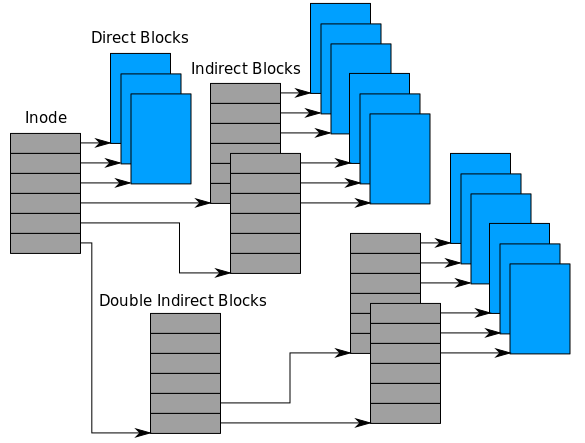
\includegraphics[width=.8\linewidth]{inode.png}
\end{center}
\end{frame}

\begin{frame}
\frametitle{Fast File System}
\begin{itemize}
  \item Fast File System - первая из классических Unix-овых ФС, в которой были
  учтены особенности диска
  \begin{itemize}
    \item не то, чтобы до этого никто не заботился о производительности;
    \item но ребята из Berkely, которые создали FFS довольно буедительно
    показали, что диск в ФС того времени использовался неэффективно.
  \end{itemize}
  \item В Fast File System минимальный размер блока - 4Kb
  \begin{itemize}
    \item т. е. за одно обращение к диску ФС пишет/читаете сразу 8 секторов;
    \item это привело к заметному увеличению скорости работы ФС, что ясно
    показало, что другими ФС диск использовался не эффективно.
  \end{itemize}
\end{itemize}
\end{frame}

\begin{frame}
\frametitle{Цилиндровые группы}
\begin{itemize}
  \item Цилиндровая группа - группа блоков, которые расположены на диске рядом
  \begin{itemize}
    \item цилиндровые группы - еще одна оптимизация введенная в FFS;
    \item каждая цилиндровая группа содержит свой набор Inode-ов, битовую карту
    свободных/занятых блоков внутри группы и прочее.
  \end{itemize}
  \item Цилиндровые группы используются для более эффективной аллокации ресурсов
  на диске:
  \begin{itemize}
    \item достаточно большие куски файла пытаются положить в одну цилиндровую
    группу;
    \item Inode-ы файлов в одном каталоге, стараются также положить в одну
    цилиндровую группу;
    \item при этом стараемся не заполнять цилинддровые группы под завязку.
  \end{itemize}
\end{itemize}
\end{frame}

\begin{frame}
\frametitle{Классические Unix-овые ФС}
\begin{itemize}
  \item FFS - это предшественник классических Unix-овых ФС
  \begin{itemize}
    \item сейчас никто не использует FFS (скорее всего), но многие пользуются
    ее наследниками: ext3 и ext4 (ext2, если кто-то ей пользуется).
  \end{itemize}
  \item Многие детали отличаются, но многие идеи остаются:
  \begin{itemize}
    \item например, каталог это не просто набор записей, а HTree/B+-tree или
    какая-то подобная индексная структура данных;
    \item журналирование для обеспечения консистентности вместо soft updates;
    \item а цилиндровые группы остались, хотя возможно называются по-другому.
  \end{itemize}
\end{itemize}
\end{frame}


  \begin{frame}
  \begin{center}
  \Huge Q\&A
  \end{center}
  \end{frame}
\end{document}
